

\documentclass[./Thick_TQFTs_and_Quantum_Information.tex]{subfiles}

\begin{document}

\begin{figure}[H]
\begin{center}
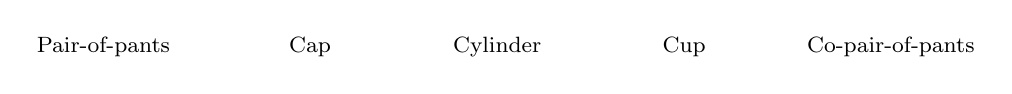
\begin{tikzpicture}[scale=0.25]
\pants{(0, 0)}
\node at (0, -5) {\footnotesize Pair-of-pants};
\capcob{(12, 0)}
\node at (10.5, -5) {\footnotesize Cap};
\idcob{(20, 0)}
\node at (20, -5) {\footnotesize Cylinder};
\cupcob{(28, 0)}
\node at (29.5, -5) {\footnotesize Cup};
\copants{(40, 0)}
\node at (40, -5) {\footnotesize Co-pair-of-pants};
\end{tikzpicture}
\caption{Generating Thick Tangles}
\end{center}
\end{figure}

Let $\M_n$ be the set of $n \times n$ matrices with complex entries equipped
with a multiplication:
\begin{eqnarray*}
  m_y :& \M_n \otimes \M_n &\to     \M_n \\
      :&  a   \otimes b    &\mapsto yab
\end{eqnarray*}
for some non-zero $y \in \C$. It is easy to see that this is an associative,
bilinear multiplication on $\M_n$ with unit:
\begin{eqnarray*}
  e_y :& \C &\to     \M_n \\
    :&  1 &\mapsto y^{-1}I_n
\end{eqnarray*}
where $I_n$ is the $n \times n$ identity matrix. We define
$w_y : = m_y^{\dagger}$ and $c _y := e_y^{\dagger}$.

When $y = 1$, $m_y = m_1$ is the usual matrix multiplication with the usual
unit. In this case, $w_1$ is given by the following \cite[8]{CatQChan}:
\[
  A = \sum_{i, j} a_{ij}e_{ij}
    \mapsto \sum_{i, j} a_{ij} \sum_{k} e_{ik} \otimes e_{kj}
\]
and $c_1$ is the trace map:
\begin{eqnarray*}
  c_1 :& \M_n &\to     \C \\
      :& \sum_{i, j} a_{ij}e_{ij} &\mapsto \sum_{i} a_{ii}
\end{eqnarray*}

Let the matrices representing $m_1$ and $e_1$, seen as linear maps, be $P_1$ and
$Q_1$ respectively. It is easy to see that the matrices for $m_y$ and $e_y$ are
$P_y := yP_1$ and $Q_y = y^{-1}Q_1$ respectively, so that $m_y = ym_1$ and
$e_y = y^{-1}e_1$, for any $y \in \C$. Hence,
\begin{align*}
  w_y &= m_y^{\dagger} = \cnj{y}m_1^{\dagger} = \cnj{y}w_1 \\
  c_y &= e_y^{\dagger} = (\cnj{y})^{-1}e_1^{\dagger} = (\cnj{y})^{-1}c_1
\end{align*}

It is well known that $(m_1, e_1, w_1, c_1)$ is a normalizable dagger Frobenius
structure on $\M_n$ \cite[8, 10]{CatQChan}. Using a Frobenius law for $m_1$
and $w_1$, we observe that
\[
  (m_y \otimes \id) \circ (\id \otimes w_y)
  = (ym_1 \otimes \id) \circ (\id \otimes (\cnj{y})^{-1}w_1)
  = y(\cnj{y})^{-1}w_1m_1
  = w_ym_y
\]
which establishes a Frobenius law for $m_y$ and $w_y$. We can prove the other
Frobenius law for $m_y, w_y$ similarly, establishing the following theorem.

\begin{thm}
$\M_n$ along with $m_y, e_y, w_y, c_y$ is a dagger Frobenius algebra.
\end{thm}

By a diagram deformation applied on the definition of normalizability
\cite[9]{CatQChan}, the above algebra is normalizable if and only if there
exists a central positive definite map $\fn{z}{\M_n}{\M_n}$ satisfying:
\[
  c_ym_yw_yz^2 = c_y \iff |y|^2c_1m_1w_1z^2 = c_1
\]
We can show that $m_1w_1(a) = na$ and hence $m_yw_y(a) = y\cnj{y} (na)
= n|y|^2 a$ for all $a \in \M_n$ so that the above relation becomes:
\begin{equation}\label{simplenorm}
  c_1z^2 = \frac{1}{n|y|^2}c_1
\end{equation}
An obvious candidate for $z$ is the map $a \mapsto \frac{1}{\sqrt{n}|y|} a$.
However, we are interested in $z$ arising from a PFT. So, we define:
\begin{defn}
Let $(A, m, e, w, c)$ be a dagger Frobenius algebra defined by (or defining) a
PFT $F$. We say that $A$ is normalizable under $F$ if there exists a planar
cobordism $\fn{Z}{I}{I}$ for which $F(Z)$ is a normalizer for $A$.
\end{defn}

Let $F$ be a PFT defined by the Frobenius structure $\M_n, m_y, e_y, w_y, c_y$.
That is, if $I$, $M$, $E$, $W$, $C$ are the interval, pair-of-pants, cup (unit
for $I$ seen as a Frobenius monoid under $M$ in $2\Thick$), co-pair-of-pants and
cap (counit for $I$) respectively, then we have:
\[
  F(I) = \M_n, F(M) = m_y, F(E) = e_y, F(W) = w_y, F(C) = c_y
\]

Let $\M_{n}$ with the above structure be normalizable under $F$, with normalizer
$z = F(Z)$ for some planar cobordism $\fn{Z}{I}{I}$. Noting that every
$\fn{Z}{I}{I}$ is determined by its genus, say $k$, and that each hole
decomposes as the map $MW$, we must have that $Z = (MW)^k$. This yields
\[
  z(a) = (m_yw_y)^k(a) = n^{k}|y|^{2k}a
\]
for all $a \in \M_n$. Substituting this into the simplified normalizability
condition \eqref{simplenorm}, we get:
\begin{align*}
       & c_1(z^2(a)) = \frac{1}{n|y|^2} c_1(a)\\
  \iff & n^{2k}|y|^{4k} c_1(a) = \frac{1}{n|y|^2} c_1(a)\\
  \iff & |y|^{4k + 2}c_1(a) = \frac{1}{n^{2k + 1}} c_1(a)
\end{align*}
Since $a$ is arbitrary, we can choose $a = e_{11}$ so that the above relation
becomes:
\[
  |y|^{2(2k + 1)} = \frac{1}{n^{2k + 1}}
  \iff |y| = \frac{1}{\sqrt{n}}
\]

We note that if this is true, then it it so, regardless of the genus of $Z$ --
this is unsurprising because:
\[
  z(a) = n^k|y|^{2k} a = n^k \br{n^{-1/2}}^{2k} a = a
\]
so that $z$ must be the identity. We collect these results as follows.
\begin{thm}\label{pftnorm}
The dagger Frobenius algebra $(\M_n, m_y, e_y, w_y, c_y)$ is normalizable under
a PFT if and only if $|y| = n^{-1/2}$. In this case, $F(Z)$ is a normalizer for
every planar cobordism $\fn{Z}{I}{I}$ in $2\Thick$ and must be be the identity
map $\M_n \to \M_n$.
\end{thm}
\begin{proof}
If $z = F(Z)$ for some PFT $F$ and some planar cobordism $Z$ in $2\Thick$, then
we have shown above that $|y| = n^{-1/2}$. If, on the other hand,
$|y| = n^{-1/2}$, then we can set $Z = (MW)^k$ for any $k \in \N \cup \set{0}$
and $z = F(Z)$. In this case, using the decomposition of a hole as $MW$, we
get:
\[
  c_1(z^2(a)) = c_1(n^k|y|^{2k} a) = n^k \frac{1}{n^k} c_1(a) = c_1(a)
    = \frac{1}{n \frac{1}{(\sqrt{n})^2}} c_1(a)
    = \frac{1}{n|y|^2} c_1(a)
\]
Thus, $F(Z)$ is a normalizer for the given dagger Frobenius structure. That
$F(Z)$ must be the identity was shown before.
\end{proof}

\begin{cor}
Not all normalizable dagger Frobenius algebras are accounted for by PFTs.
\end{cor}
\begin{proof}
$(\M_n, m_1, e_1, w_1, c_1)$ is a normalizable dagger Frobenius algebra with
normalizer $a \mapsto n^{-1/2} a$ but this normalizer cannot be not in the
image of a PFT $F$.
\end{proof}

We do not wish to give up just yet. We let $\M_{n, y}$ denote the dagger
Frobenius algebra $(\M_n, m_y, e_y, w_y, c_y)$ and consider the map
$\phi : \M_{n, y} \to \M_{n, 1} : a \mapsto \alpha a$, for some non-zero
$y, \alpha \in \C$ and observe that
\[
  \phi m_y(a \otimes b) = \phi(yab) = y\phi(ab) = y\alpha ab
\]
and
\[
  m_1(\phi(a) \otimes \phi(b)) = \alpha^2 ab
\]
For phi to be an algebra homomorphism, we need $\alpha^2 = y\alpha \iff y =
\alpha$. Indeed, we see that, under phi,
\[
  y^{-1}I_n \mapsto I_n
\]
showing unitality. Invertibility being clear, $\phi$ is an algebra isomorphism.
We observe the interaction of $\phi$ with the dagger structure:
\[
  \phi(a^{\dagger}) = ya^{\dagger} = (\cnj{y}a)^{\dagger} =
    \frac{y}{\cnj{y}}\phi(a)^{\dagger}
\]
If $y$ is real, then $\phi$ is a $*$--isomophism.
\begin{thm}
Every $\M_{n, 1}$ is $*$--isomorphic to $\M_{n, y}$ for some real $y$.
\end{thm}

If $\M_{n, y}$ is normalizable under a PFT, then for every $\fn{Z}{I}{I}$,
$F(Z) = \id_{\M_{n, y}}$ is a normalizer for $\M_{n, y}$ and
$\phi \circ F(Z) = \phi$. Furthermore, $|y| = n^{-1/2}$ by \ref{pftnorm}.
Finally, if $y$ is real, making $\phi$ a $*$--isomorphism as above, we must have
$y = \pm n^{-1/2}$. Picking the positive value for $y$,
$\phi \circ F(Z) = \phi$ seen as map $\M_{n, 1} \to \M_{n, 1}$ is the usual
normalizer for $\M_{n, 1}$.

I am guessing that this argument generalizes to direct sums of the form
$\bigoplus_{i = 1}^r \M_{n_i}$ as in \cite[10]{CatQChan}.  If this is true, we
may have characterized the normalizability of finite dimensional $C^*$--algebras
through PFTs up to $*$--isomorphism, since normalizable dagger Frobenius
algebras over $\C$ are precisely the finite direct sums of finite dimensional
matrix algebras (up to $*$--isomorphism?). In other words, if the above is
correct, then
\begin{thm}
Every finite dimensional $C^*$--algebra is $*$--isomorphic to a dagger Frobenius
algebra normalizable under a PFT with the ismorphism ``carrying over the
normalizer''\footnote{in some sense} both ways.
\end{thm}

If we are satisfied with the above, we may also look at the $\text{CP}^*$
condition or complete-positivity of mappings between $C^*$ algebras and their
relations with monoidal natural transformations between PFTs.

\end{document}

